% LaTeX source for ``การเรียนรู้ของเครื่องสำหรับเคมีควอนตัม (Machine Learning for Quantum Chemistry)''
% Copyright (c) 2022 รังสิมันต์ เกษแก้ว (Rangsiman Ketkaew).

% License: Creative Commons Attribution-NonCommercial-NoDerivatives 4.0 International (CC BY-NC-ND 4.0)
% https://creativecommons.org/licenses/by-nc-nd/4.0/

%--------------------------
\chapter{ออร์บิทัลของอะตอมไฮโดรเจน}
\label{ch:hydro_orbitals}
%--------------------------

%--------------------------
\section{ฟังก์ชันคลื่นของอะตอมไฮโดรเจน}
\label{sec:hydro_wfn}
%--------------------------
\idxboth{ฟังก์ชันคลื่น!ออร์บิทัลของอะตอมไฮโดรเจน}{Wavefunction!Hydrogen Orbital}

ในหัวข้อนี้ผู้อ่านจะได้เรียนรู้วิธีการเขียนโค้ดด้วยภาษา Python สำหรับการพล็อตรูปร่างของ Wavefunction หรือออร์บิทัลของอะตอมไฮโดรเจน 
ก่อนอื่นนั้นเราจะต้องมาทำความเข้าใจกับสมการ Wavefunction ของอะตอมไฮโดรเจนที่มี 1 อิเล็กตรอนกันก่อน โดยมีสมการดังต่อไปนี้

\begin{equation}\label{eq:hydro_wfn}
    \psi_{nlm}(r,\theta,\phi) = R_{nl}(r) Y_{lm}(\theta,\phi)
\end{equation}

\noindent ซึ่งเป็นผลคูณระหว่างส่วนที่เป็นเชิงรัศมี (Radial Part) หรือ $R_{nl}(r)$ และส่วนที่เป็นเชิงมุม (Angular Part) หรือ 
$Y_{lm}(\theta, \phi$ ตามลำดับ โดยมีสมการที่เป็นฟังก์ชันของเลขควอนตัมดังต่อไปนี้

\begin{equation}\label{eq:hydro_wfn_rad}
    R_{nl}(r) = \sqrt{\Big(\frac{2}{n a_0}\Big)^3 \frac{(n-l-1)!}{2n (n+l)!}} e^{-r/n a_0} 
        \Big( \frac{2r}{na_0}\Big)^l  \cdot L^{2l+1}_{n-l-1} \Big(\frac{2r}{n a_0} \Big)
\end{equation}

\noindent และ

\begin{equation}\label{eq:hydro_wfn_ang}
    Y_{lm}(\theta,\phi) = \Theta_{lm}(\theta) \Phi_m (\phi) 
        = \sqrt{\frac{2l+1}{4\pi} \frac{(l-m)!}{(l+m)!} } 
        P_{lm}(cos \theta) \cdot e^{im\phi}
\end{equation}

โดยในขั้นตอนการพล็อต Wavefunction นั้นเราจะทำการสร้างฟังก์ชันสำหรับ $R_{nl}(r)$ และ $Y_{lm}(\theta, \phi$ ตามลำดับ
แล้วหลังจากนั้นก็นำมาร่วมกันเพื่อพล็อตเป็นออร์บิทัลในปริภูมิ 3 มิติต่อไป

\noindent \textbf{หมายเหตุ} 
\begin{enumerate}[topsep=0pt,noitemsep]
    \item เราพิจารณาส่วนจริง (Real Part) ของ Psherical Harmonics ของ Wavefunction เท่านั้น โดยเราจะไม่พิจารณาส่วนจินตภาพ 
    (Imaginary Part)

    \item เราจะใช้ Atomic Units สำหรับปริมาณดังต่อไปนี้เพื่อความสะดวกในการเขียนโค้ด $a_0=1, \hbar=1, m_e=1, e=1$
\end{enumerate}

%--------------------------
\section{การเขียนโค้ดสำหรับพล็อตออร์บิทัล}
\label{sec:code_hydro_wfn}
%--------------------------

ผู้เขียนแนะนำให้ผู้อ่านใช้ IPython-based Platform สำหรับเขียนโค้ด เช่น Jupyter Notebook

\bigskip

$\bullet$ \textbf{เตรียมไลบรารี่}

\begin{lstlisting}[style=MyPython]
%matplotlib inline
import matplotlib.pyplot as plt

from matplotlib import cm, colors
from mpl_toolkits.mplot3d import Axes3D

import numpy as np
import scipy.integrate as integrate

# Increase resolution for retina display
from IPython.display import set_matplotlib_formats
set_matplotlib_formats('retina')

# Load interactive widgets
import ipywidgets as widgets
import ipyvolume as ipv
\end{lstlisting}

\noindent ถ้าหากผู้อ่านยังไม่ได้ติดตั้งไลบรารี่สามารถติดตั้งได้โดยใช้คำสั่ง

\begin{lstlisting}[style=MyBash]
pip install LIBRARY_NAME
\end{lstlisting}

\bigskip

$\bullet$ \textbf{พล็อต Radial Part ของ Wavefunction}

เริ่มต้นด้วยการสร้างฟังก์ชันสำหรับ Radial Part ของ Wavefunction ซึ่งเราจะใช้พหุนามลาแกร์ (Laguerre Polynomials) โดยกำหนดให้ 
$n = 0$ และ $l = =$ เป็นค่าเริ่มต้น

\begin{lstlisting}[style=MyPython]
def psi_R(r, n=1, l=0):
    coeff = np.sqrt((2.0/n)**3 * spe.factorial(n-l-1) /(2.0*n*spe.factorial(n+l)))
    laguerre = spe.assoc_laguerre(2.0*r/n,n-l-1,2*l+1)
    
    return coeff * np.exp(-r/n) * (2.0*r/n)**l * laguerre
\end{lstlisting}

\noindent ทำการกำหนด Grid Space สำหรับการพล็อตค่าของ Radial Part

\begin{lstlisting}[style=MyPython]
r = np.linspace(0, 100, 1000)
R = psi_R(r, n=5, l=1)

plt.plot(r, R**2, lw=3)
plt.xlabel('$r [a_0]$',fontsize=20)
plt.ylabel('$R_{nl}(r)$', fontsize=20)
plt.grid('True')
\end{lstlisting}

\begin{figure}[H]
    \centering
    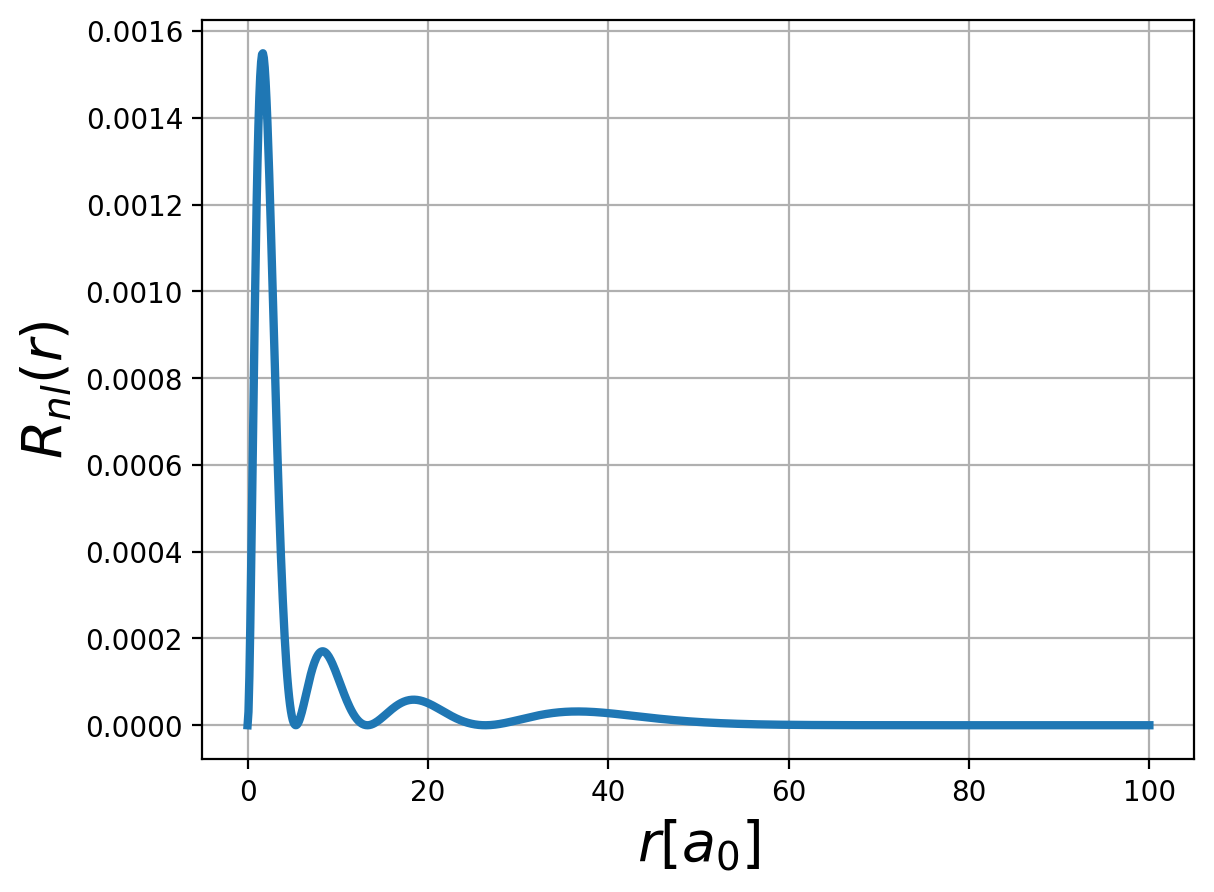
\includegraphics[width=0.8\linewidth]{fig/wfn_hydro_radial.png}
    \caption{Radial Part สำหรับ $n = 5$ และ $l = 0$}
    \label{fig:wfn_hydro_radial}
\end{figure}

\noindent โดยจะได้พล็อตตามภาพที่ \ref{fig:wfn_hydro_radial} ขั้นตอนต่อไปคือทำการเพิ่ม Interactive Widget สำหรับพล็อตที่%
สามารถปรับค่าเลขควอนตัมได้

\begin{lstlisting}[style=MyPython]
nmax=10

@widgets.interact(n = np.arange(1, nmax, 1), l = np.arange(0, nmax-1, 1))

def plot_radial(n=1, l=0):
    r = np.linspace(0,250,10000)
    psi2 = psi_R(r,n,l)**2 * (r**2)
    plt.plot(r, psi2, lw=2, color='red')

    # Styling the plot
    plt.xlabel('$r [a_0]$')
    plt.ylabel('$R_{nl}(r)$')
    rmax = n**2*(1+0.5*(1-l*(l+1)/n**2))
    plt.xlim([0, 2*rmax])
\end{lstlisting}

\begin{figure}[H]
    \centering
    \begin{subfigure}{0.5\textwidth}
        \centering
        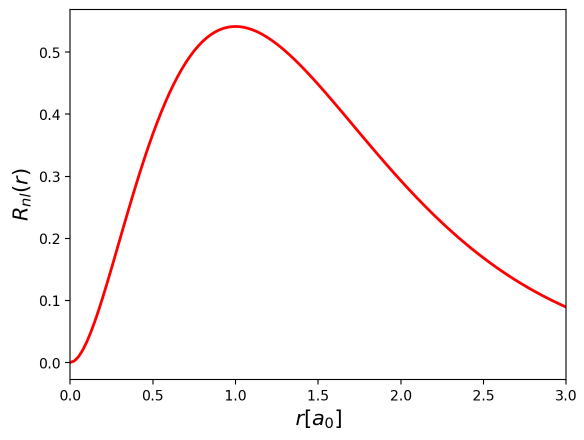
\includegraphics[width=0.9\linewidth]{fig/wfn_hydro_radial_n1_l0.png}
        \caption{$n = 1$ และ $l = 0$}
        \label{fig:wfn_hydro_radial_n1_l0}
    \end{subfigure}%
    \begin{subfigure}{0.5\textwidth}
        \centering
        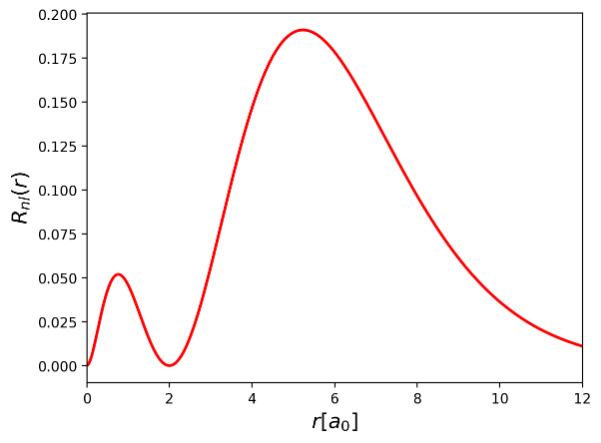
\includegraphics[width=0.9\linewidth]{fig/wfn_hydro_radial_n2_l0.png}
        \caption{$n = 2$ และ $l = 0$}
        \label{fig:wfn_hydro_radial_n2_l0}
    \end{subfigure}
    \\
    \vspace{1em}
    \begin{subfigure}{0.5\textwidth}
        \centering
        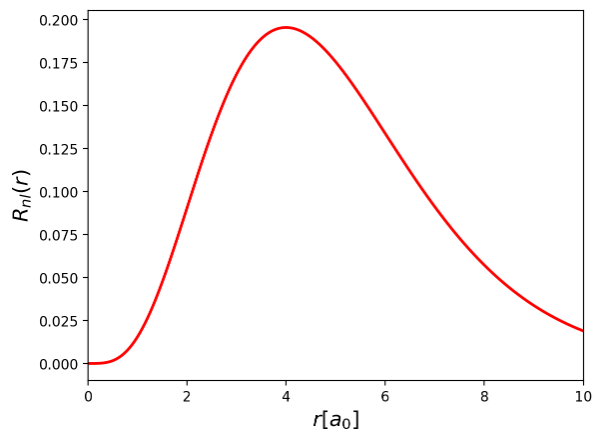
\includegraphics[width=0.9\linewidth]{fig/wfn_hydro_radial_n2_l1.png}
        \caption{$n = 2$ และ $l = 1$}
        \label{fig:wfn_hydro_radial_n2_l1}
    \end{subfigure}%
    \begin{subfigure}{0.5\textwidth}
        \centering
        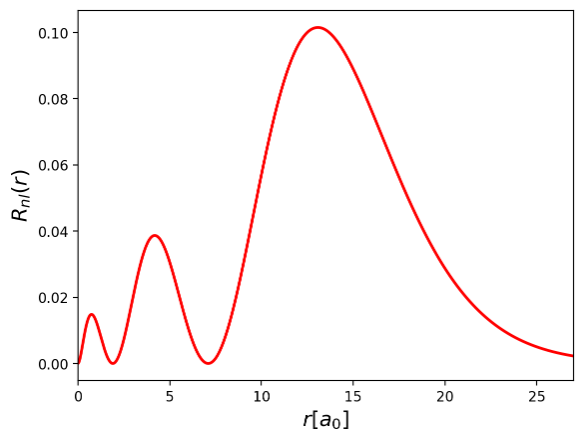
\includegraphics[width=0.9\linewidth]{fig/wfn_hydro_radial_n3_l0.png}
        \caption{$n = 3$ และ $l = 0$}
        \label{fig:wfn_hydro_radial_n3_l0}
    \end{subfigure}
    \\
    \vspace{1em}
    \begin{subfigure}{0.5\textwidth}
        \centering
        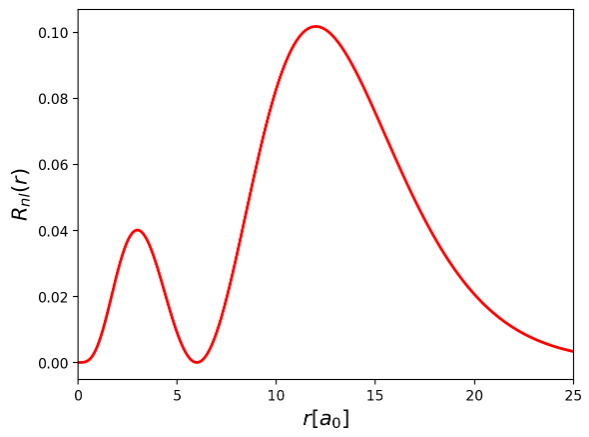
\includegraphics[width=0.9\linewidth]{fig/wfn_hydro_radial_n3_l1.png}
        \caption{$n = 3$ และ $l = 1$}
        \label{fig:wfn_hydro_radial_n3_l1}
    \end{subfigure}%
    \begin{subfigure}{0.5\textwidth}
        \centering
        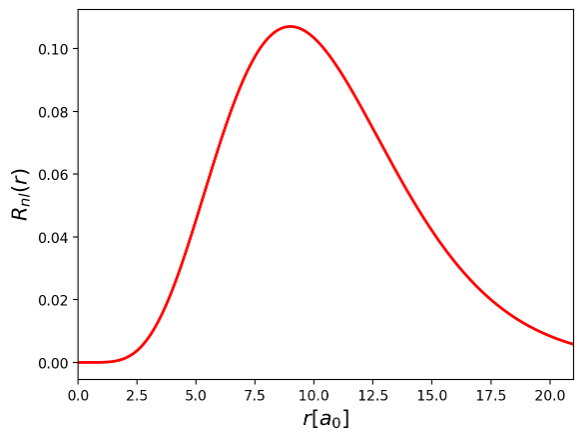
\includegraphics[width=0.9\linewidth]{fig/wfn_hydro_radial_n3_l2.png}
        \caption{$n = 3$ และ $l = 2$}
        \label{fig:wfn_hydro_radial_n3_l2}
    \end{subfigure}
    \caption{Radial Part ของ Wavefunction ของอะตอมไฮโดรเจน}
    \label{fig:wfn_hydro_radial_all}
\end{figure}

\bigskip

$\bullet$ \textbf{พล็อต Angular Part ของ Wavefunction}

สร้างฟังก์ชันสำหรับสร้าง Angular Part (สนใจเฉพาะส่วนจริงเท่านั้น) เช่นเดียวกันกับ Radial Part

\begin{lstlisting}[style=MyPython]
def psi_ang(phi,theta, l=0, m=0):
    sphHarm = spe.sph_harm(m,l,phi,theta)
    
    return sphHarm.real
\end{lstlisting}

\vspace{1em}
\noindent ทำการสร้าง Grid Space สำหรับการพล็อต Spherical Harmonics แบบ 3 มิติ

\begin{lstlisting}[style=MyPython]
phi, theta = np.linspace(0, np.pi, 100), np.linspace(0, 2*np.pi, 100)
phi, theta = np.meshgrid(phi, theta)
Ylm = psi_ang(theta,phi,l=2,m=0)
\end{lstlisting}

\vspace{1em}
\noindent ทำการกำหนดค่าเริ่มต้น Domain สำหรับการพล็อตออร์บิทัล นั่นคือ $x$ กับ $y$ แล้วทำการคำนวณค่ามุม Angular Part $z$ 
สำหรับแต่ละจุดบน Grid

\begin{lstlisting}[style=MyPython]
x = np.sin(phi) * np.cos(theta) * abs(Ylm)
y = np.sin(phi) * np.sin(theta) * abs(Ylm)
z = np.cos(phi) * abs(Ylm)
\end{lstlisting}

\vspace{1em}
\noindent ทำการกำหนดตั้งค่าสำหรับการพล็อตแบบ 3 มิติ โดยกำหนดให้ \pyinline{projection='3d'} สำหรับ Matplotlib

\begin{lstlisting}[style=MyPython]
# Set up the 3D Canvas
fig = plt.figure(figsize=(10,10))
ax = fig.add_subplot(111, projection='3d')

# Normalize color bar to [0,1] scale
fcolors = (Ylm - Ylm.min())/(Ylm.max() - Ylm.min())

# Make 3D plot of real part of spherical harmonic
ax.plot_surface(x, y, z, facecolors=cm.seismic(fcolors), alpha=0.3)

# Project 3D plot onto 2D planes
cset = ax.contour(x, y, z,20, zdir='z',offset = -1, cmap='summer')
cset = ax.contour(x, y, z,20, zdir='y',offset =  1, cmap='winter' )
cset = ax.contour(x, y, z,20, zdir='x',offset = -1, cmap='autumn')

# Set axes limit to keep aspect ratio 1:1:1
ax.set_xlim(-1, 1)
ax.set_ylim(-1, 1)
ax.set_zlim(-1, 1)
\end{lstlisting}

\begin{figure}[H]
    \centering
    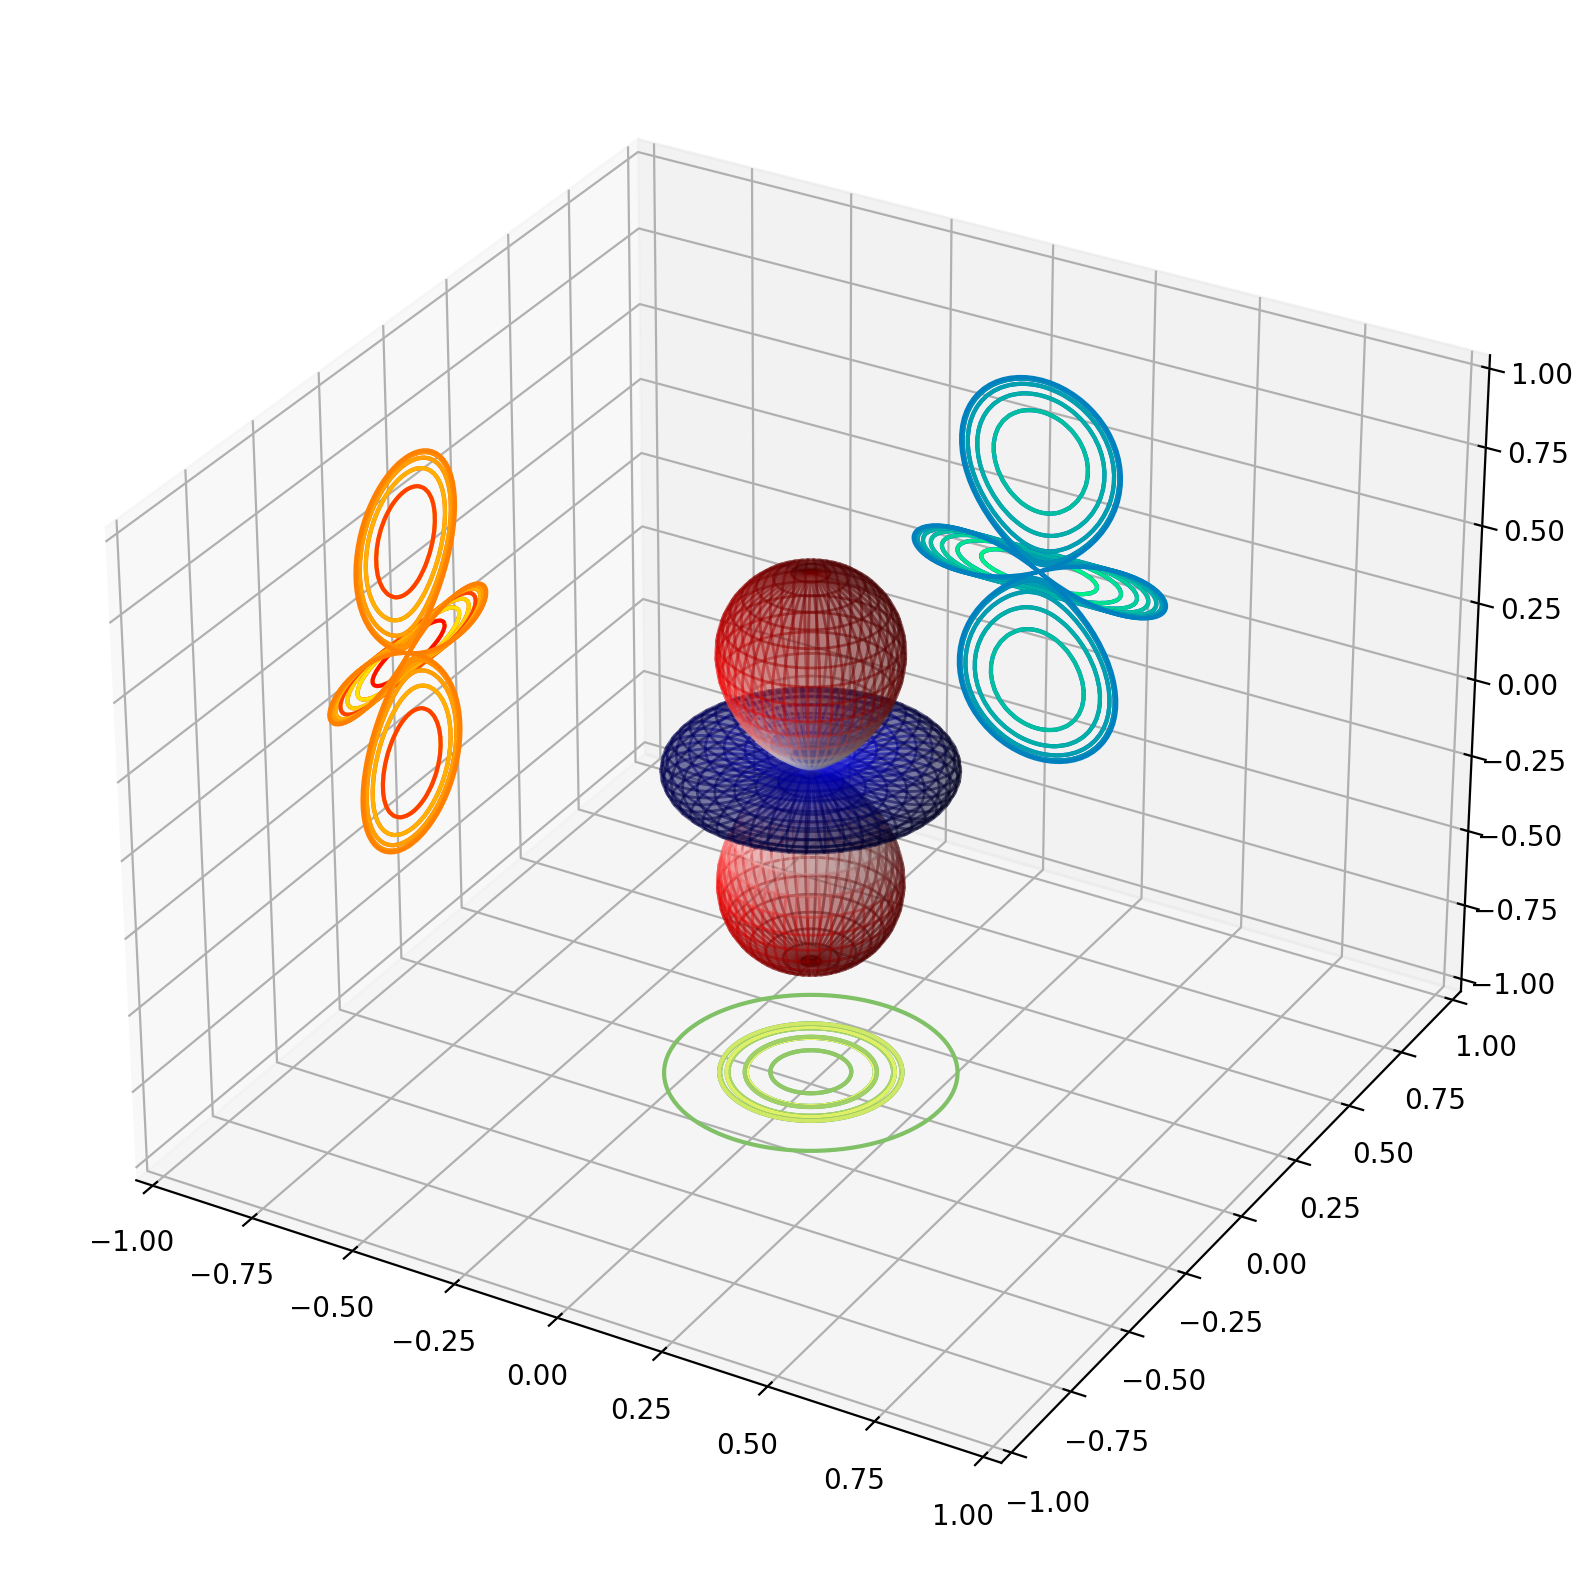
\includegraphics[width=0.9\linewidth]{fig/wfn_hydro_angular.png}
    \caption{Angular Part สำหรับ $l = 2$ และ $m = 0$}
    \label{fig:wfn_hydro_angular}
\end{figure}

\bigskip

$\bullet$ \textbf{รวม Radial Part และ Angular Part สำหรับพล็อตออร์บิทัล}

สร้างฟังก์ชันสำหรับคำนวณ Wavefunction ของไฮโดรเจนโดยรับค่าอินพุตดังต่อไปนี้ 

\begin{itemize}[topsep=0pt,noitemsep]
    \item r: Radial Coordinate $(r)$
    
    \item theta: Polar Coordinate $(\theta)$
    
    \item phi: Azimuthal Coordinate $(\phi)$
    
    \item n: Principle Quantum Number $(n)$
    
    \item l: Angular Momentum Quantum Number $(l)$
    
    \item m: Magnetic Quantum Number $(m)$
\end{itemize}

\noindent แล้วทำการคืนค่าออกมาเป็น Wavefunction ซึ่งได้จากผลคูณระหว่าง $\psi_{R}$ และ $\psi_{\text{ang}}$

\begin{lstlisting}[style=MyPython]
def HFunc(r, theta, phi, n, l, m):
    # Hydrogen wavefunction // a_0 = 1

    return psi_R(r, n, l) * psi_ang(phi, theta, l,m)
\end{lstlisting}

\vspace{1em}
\noindent กำหนดค่าเริ่มต้นของเลขควอนตัมหลักและเลขควอนตัมเชิงมุม เช่น กำหนดค่าสูงสุดคือ 10 ซึ่งเมื่อทำการพล็อตแล้วเราสามารถเปลี่ยนค่า
$n$, $l$, และ $m$ ได้ตามต้องการเพราะว่าเราใช้ Interactive Plot

\begin{lstlisting}[style=MyPython]
nmax = 10
lmax = nmax-1

@widgets.interact(n=np.arange(1,nmax,1), l = np.arange(0,nmax-1,1), m=np.arange(-lmax,lmax+1,1))

def psi_xz_plot(n=1, l=0, m=0):
    plt.figure(figsize=(10, 8))
    limit = 4*(n+l)
    x_1d = np.linspace(-limit, limit, 500)
    z_1d = np.linspace(-limit, limit, 500)
    x,z = np.meshgrid(x_1d, z_1d)
    y   = 0
    
    r = np.sqrt(x**2 + y**2 + z**2)
    theta = np.arctan2(np.sqrt(x**2+y**2), z)
    phi = np.arctan2(y, x)
    psi_nlm = HFunc(r,theta,phi,n,l,m)
    
    # Try cmap = inferno, rainbow, autumn, summer
    # plt.pcolormesh(x, z, psi_nlm, cmap='inferno')
    plt.contourf(x, z, psi_nlm, 20, cmap='seismic', alpha=0.6) # Classic orbitals
    plt.colorbar()
    plt.title(f"$n, l, m={n,l,m}$", fontsize=20)
    plt.xlabel('X', fontsize=20)
    plt.ylabel('Z', fontsize=20)
\end{lstlisting}

\medskip

\begin{figure}[H]
    \centering
    \begin{subfigure}{0.5\textwidth}
        \centering
        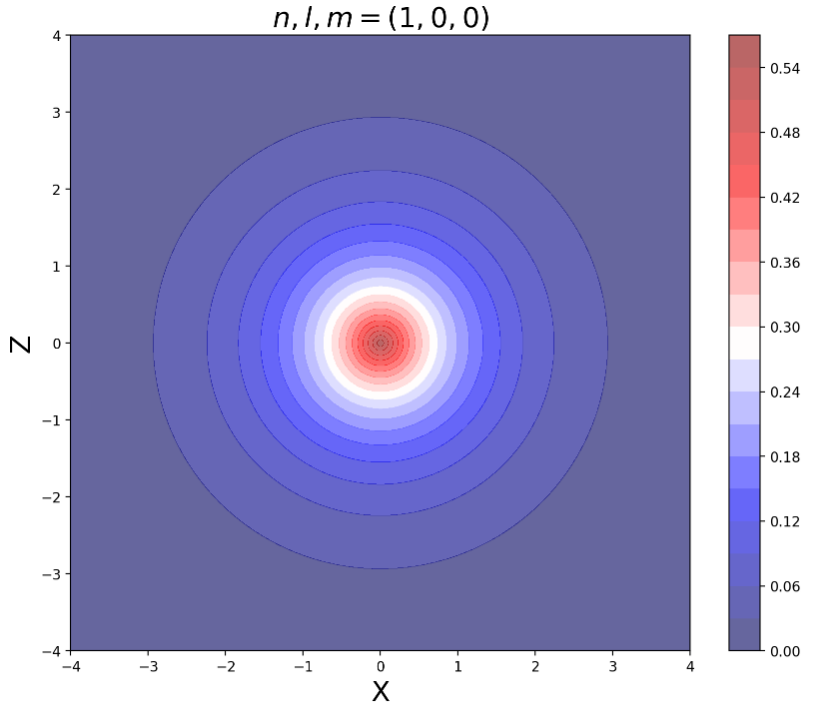
\includegraphics[width=0.9\linewidth]{fig/wfn_hydro_n1_l0_m0.png}
        \caption{$n = 1$, $l = 0$, และ $m = 0$}
        \label{fig:wfn_hydro_n1_l0_m0}
    \end{subfigure}%
    \begin{subfigure}{0.5\textwidth}
        \centering
        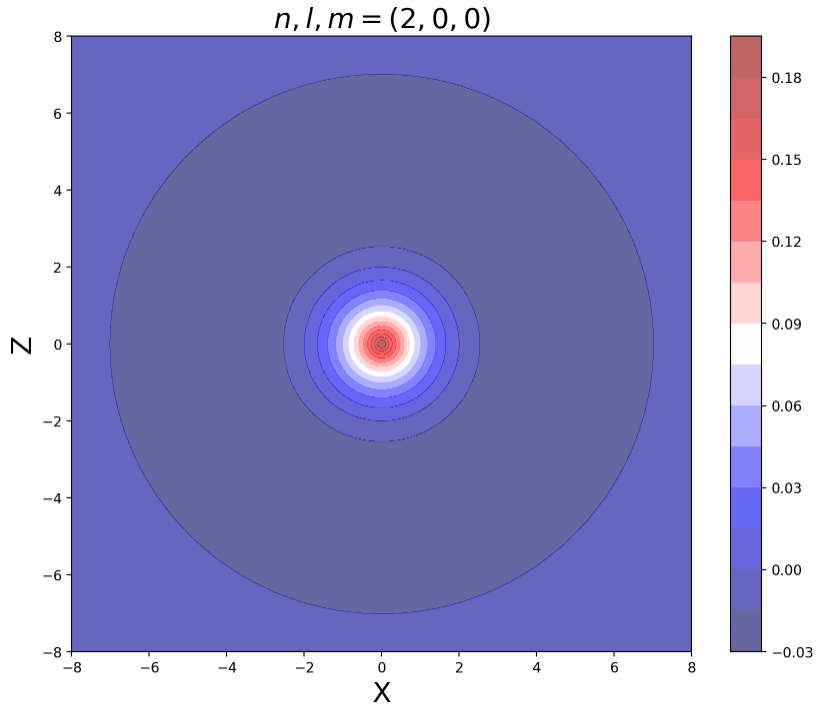
\includegraphics[width=0.9\linewidth]{fig/wfn_hydro_n2_l0_m0.png}
        \caption{$n = 2$, $l = 0$, และ $m = 0$}
        \label{fig:wfn_hydro_n2_l0_m0}
    \end{subfigure}
    \\
    \vspace{1em}
    \begin{subfigure}{0.5\textwidth}
        \centering
        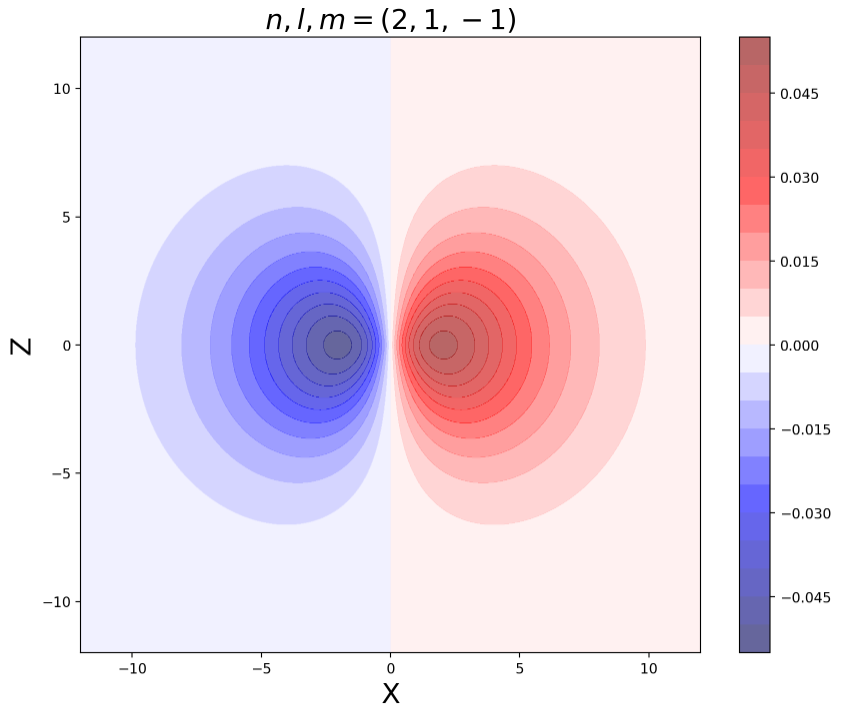
\includegraphics[width=0.9\linewidth]{fig/wfn_hydro_n2_l1_m-1.png}
        \caption{$n = 2$, $l = 1$, และ $m = -1$}
        \label{fig:wfn_hydro_n2_l1_m-1}
    \end{subfigure}%
    \begin{subfigure}{0.5\textwidth}
        \centering
        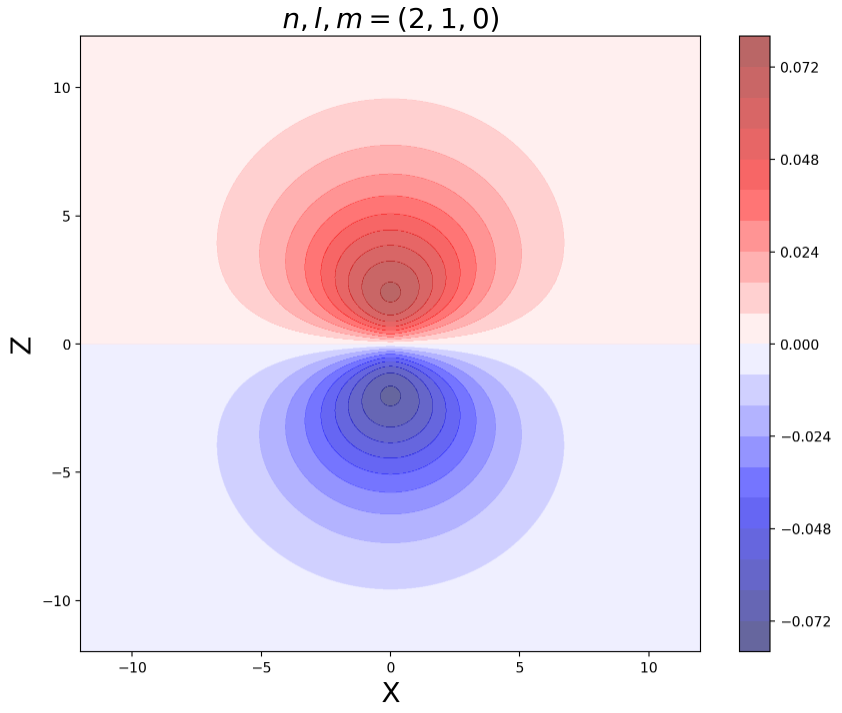
\includegraphics[width=0.9\linewidth]{fig/wfn_hydro_n2_l1_m0.png}
        \caption{$n = 2$, $l = 1$, และ $m = 0$}
        \label{fig:wfn_hydro_n2_l1_m0}
    \end{subfigure}
    \\
    \vspace{1em}
    \begin{subfigure}{0.5\textwidth}
        \centering
        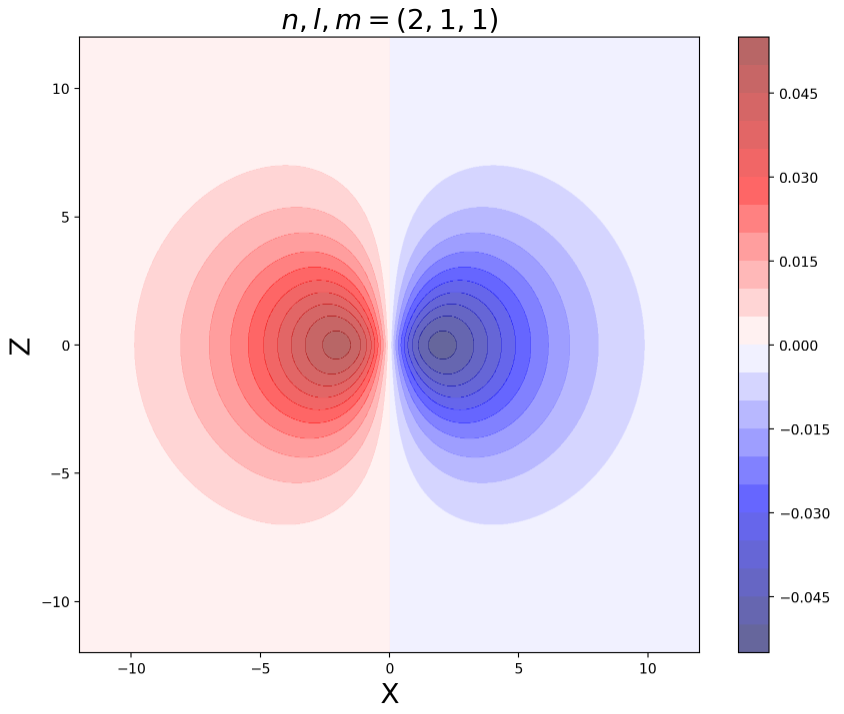
\includegraphics[width=0.9\linewidth]{fig/wfn_hydro_n2_l1_m1.png}
        \caption{$n = 2$, $l = 1$, และ $m = 1$}
        \label{fig:wfn_hydro_n2_l1_m1}
    \end{subfigure}%
    \begin{subfigure}{0.5\textwidth}
        \centering
        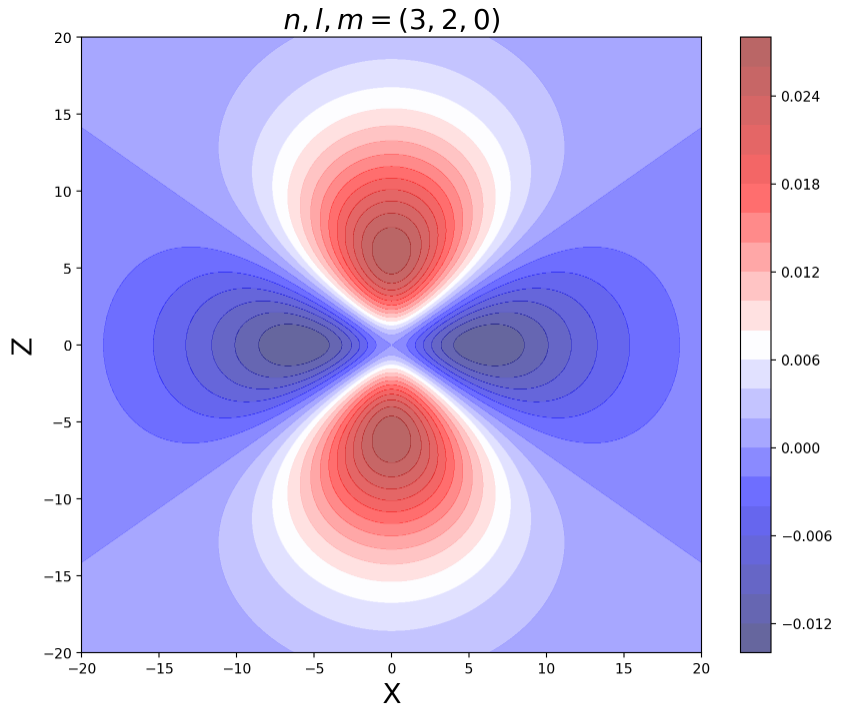
\includegraphics[width=0.9\linewidth]{fig/wfn_hydro_n3_l2_m0.png}
        \caption{$n = 3$, $l = 2$, และ $m = 0$}
        \label{fig:wfn_hydro_n3_l2_m0}
    \end{subfigure}
    \caption{Wavefunction ของอะตอมไฮโดรเจน ซึ่งรวม Radial และ Angular Part เข้าด้วยกัน}
    \label{fig:wfn_hydro_all}
\end{figure}

\noindent คำนวณค่าสำหรับการพล็อตออร์บิทัลแบบสมบูรณ์แบบ Interactive

\begin{lstlisting}[style=MyPython]
# Variables to adjust
maxi = 60
resolution = 160

base = np.linspace(-maxi, maxi, resolution)[:, np.newaxis, np.newaxis]
x2 = np.tile(base, (1, resolution, resolution))
y2 = np.swapaxes(x2, 0, 1)
z2 = np.swapaxes(x2, 0, 2)

total = np.concatenate((x2[np.newaxis,:], y2[np.newaxis,:], z2[np.newaxis,:]), axis=0)

r2 = np.linalg.norm(total, axis=0)
# Alternative theta calculation
# theta3 = np.abs(np.arctan2(np.linalg.norm(total[:2], axis=0), -total[2]))

np.seterr(all='ignore')
phi2 = np.arctan(np.divide(total[2], np.linalg.norm(total[:2], axis=0))) + np.pi/2
theta2 = np.arctan2(total[1], total[0])
\end{lstlisting}

\noindent ทำการพล็อต Wavefunction แบบสมบูรณ์

\begin{lstlisting}[style=MyPython]
ipv.figure()
psi = HFunc(r2,theta2,phi2,2,1,1)
ipv.volshow(r2**2 * np.sin(phi2)*psi**2)
ipv.show()
\end{lstlisting}

\begin{figure}[H]
    \centering
    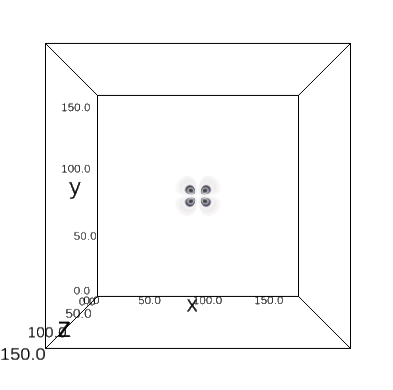
\includegraphics[width=0.8\linewidth]{fig/wfn_hydro_3d_n2_l1_m1.png}
    \caption{ออร์บิทัลของอะตอมไฮโดรเจนในปริภูมิ 3 มิติ สำหรับ $n = 2$, $l = 1$ และ $m = 1$}
    \label{fig:wfn_hydro_3d_n2_l1_m1}
\end{figure}

\noindent เรายังสามารถตรวจสอบขนาดของ Array ของข้อมูลที่ใช้ในการพล็อต Wavefunction ได้ ดังนี้

\begin{lstlisting}[style=MyPython]
psi.shape
# Output
(160, 160, 160)
\end{lstlisting}

\bigskip

จากตัวอย่างโค้ดข้างต้นจะพบว่าจริง ๆ แล้วการแสดง Wavefunction หรือออร์บิทัลที่แสดงความน่าจะเป็นหรือโอกาสที่จะพบอิเล็กตรอนนั้นไม่ได้ซับซ้อน 
ถ้าหากเรามีฟังก์ชันคณิตศาสตร์ที่ตรงไปตรงมา เราก็สามารถเขียนโค้ดตามฟังก์ชันดังกล่าวได้เลย
